\subsection{Цель выполнения домашнего задания}\label{blockN.VariantM}
\textbf{Цель выполнения домашнего задания }-- \GoalOfResearch

%-------------------------------------------------
\subsection{Задание}
Система состоит из устройств типа $A$ и типа $B$, интенсивности отказов $\lambda_A$ и $\lambda_B$ известны.
Для функционирования системы требуется хотя бы одно устройство типа $A$ и хотя бы $N_B$ устройств типа $B$.
Общее число устройств в системе (включая резервные) – $R_A$ и $R_B$ соответственно,
причём в нормальном состоянии одновременно включены сразу $N_A$ устройств типа $A$.

Если $N$ – номер зачётной книжки, а $G$ – последняя цифра в номере группы,
то параметры системы определяются следующим образом:
\[
\begin{matrix}
    \lambda_A= G + (N \bmod 3) \\
    \lambda_B= G + (N \bmod 5) \\
    N_A= 2 + (G \bmod 2) \\
    N_B= 2 + (N \bmod 2) \\
    R_A= 4 + (G \bmod 2) \\
    R_B= 5 - (G \bmod 2)
\end{matrix}
\]

Требуется:
\begin{enumerate}
    \item нарисовать граф состояний системы;
    \item составить матрицу интенсивностей переходов;
    \item записать дифференциальные уравнения Колмогорова;
    \item аналитически решить полученную систему уравнений, исходя из того, что в начальный момент времени все устройства исправны;
    \item построить графики вероятностей нахождения системы в каждом из возможных состояний с течением времени;
    \item построить график функции надёжности системы;
    \item рассчитать математическое ожидание времени безотказной работы;
    \item провести имитационное моделирование системы в терминах непрерывных марковских цепей 100 раз, рассчитать среднее выборочное значение и стандартное отклонение времени безотказной работы системы.
\end{enumerate}
%-------------------------------------------------
\newpage
\subsection{Решение}

Рассчитаем начальные данные для выполнения домашнего задания по номеру зачетки $N = 82$ и группы $G = 4$:
\[
\begin{matrix}
    \lambda_A & = G + (N \bmod 3) = 4 + (82 \bmod 3) = & 5 \\
    \lambda_B & = G + (N \bmod 5) = 4 + (82 \bmod 5) = & 6 \\
    N_A & = 2 + (G \bmod 2) = 2 + (4 \bmod 2) = & 2 \\
    N_B & = 2 + (N \bmod 2) = 2 + (82 \bmod 2) = & 2 \\
    R_A & = 4 + (G \bmod 2) = 4 + (4 \bmod 2) = & 4 \\
    R_B & = 5 - (G \bmod 2) = 5 - (4 \bmod 2) = & 5
\end{matrix}
\]
Предположим что $S^{ab}_{cd}$ - состояние системы, где
\begin{itemize}
    \item $a$ - количество работающих устройств типа $A$, включая резервные,
    \item $b$ - количество резервных устройств типа $A$,
    \item $c$ - количество работающих устройств типа $B$, включая резервные,
    \item $d$ - количество резервных устройств типа $B$.
\end{itemize}
На рисунке \ref{graph} изображен граф состояний системы.


\begin{figure}[H]
\centerline{ 
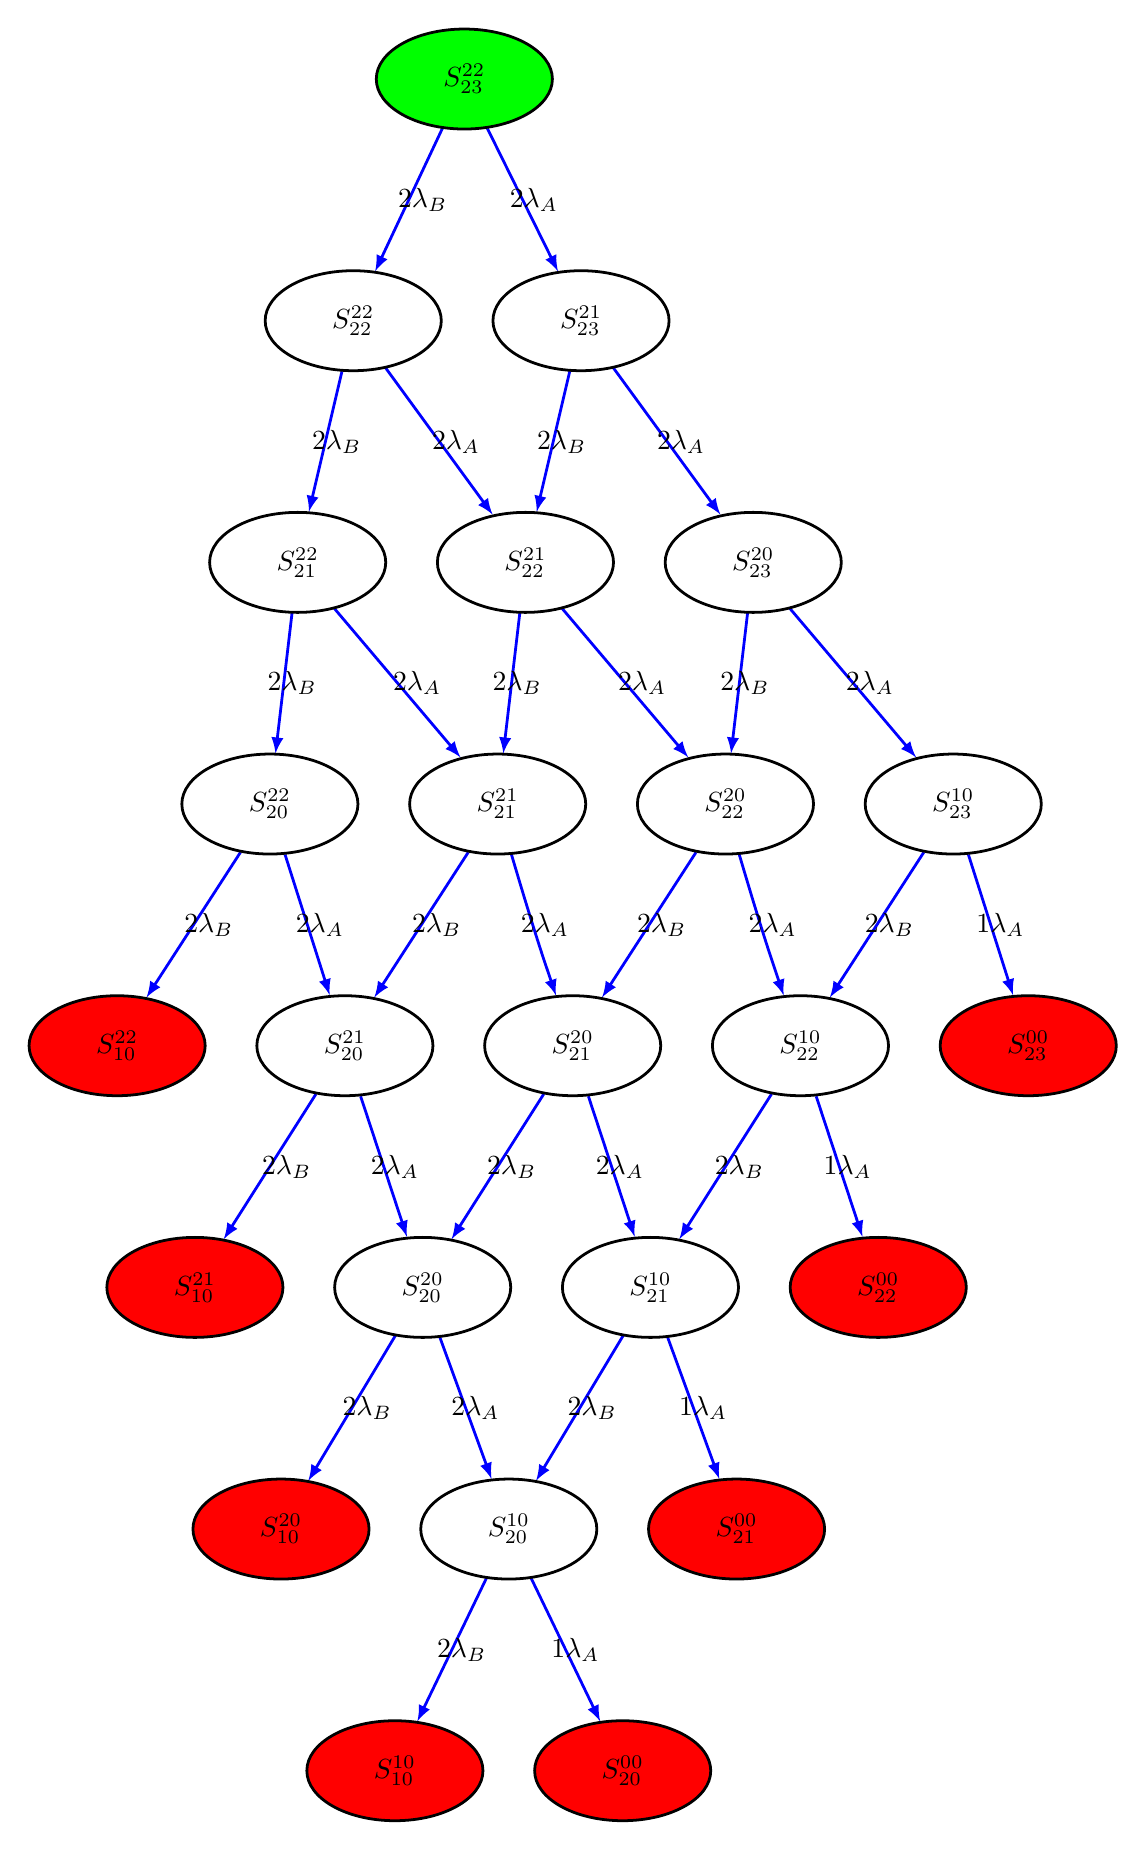
\begin{tikzpicture}[>=latex,line join=bevel,]
  \pgfsetlinewidth{1bp}
label=graph%
\pgfsetcolor{black}
  % Edge: s2223 -> s2222
  \pgfsetcolor{blue}
  \draw [->] (148.94bp,609.21bp) .. controls (143.36bp,597.33bp) and (135.75bp,581.17bp)  .. (124.73bp,557.76bp);
  \definecolor{strokecol}{rgb}{0.0,0.0,0.0};
  \pgfsetstrokecolor{strokecol}
  \draw (141.85bp,583.5bp) node {$2\lambda_B$};
  % Edge: s2223 -> s2123
  \pgfsetcolor{blue}
  \draw [->] (165.15bp,609.21bp) .. controls (171.01bp,597.33bp) and (179.0bp,581.17bp)  .. (190.57bp,557.76bp);
  \definecolor{strokecol}{rgb}{0.0,0.0,0.0};
  \pgfsetstrokecolor{strokecol}
  \draw (181.85bp,583.5bp) node {$2\lambda_A$};
  % Edge: s2222 -> s2221
  \pgfsetcolor{blue}
  \draw [->] (112.8bp,521.8bp) .. controls (110.09bp,510.28bp) and (106.46bp,494.86bp)  .. (100.89bp,471.18bp);
  \definecolor{strokecol}{rgb}{0.0,0.0,0.0};
  \pgfsetstrokecolor{strokecol}
  \draw (110.85bp,496.5bp) node {$2\lambda_B$};
  % Edge: s2222 -> s2122
  \pgfsetcolor{blue}
  \draw [->] (128.51bp,523.01bp) .. controls (137.54bp,510.63bp) and (150.23bp,493.23bp)  .. (167.03bp,470.21bp);
  \definecolor{strokecol}{rgb}{0.0,0.0,0.0};
  \pgfsetstrokecolor{strokecol}
  \draw (153.85bp,496.5bp) node {$2\lambda_A$};
  % Edge: s2123 -> s2122
  \pgfsetcolor{blue}
  \draw [->] (194.8bp,521.8bp) .. controls (192.09bp,510.28bp) and (188.46bp,494.86bp)  .. (182.89bp,471.18bp);
  \definecolor{strokecol}{rgb}{0.0,0.0,0.0};
  \pgfsetstrokecolor{strokecol}
  \draw (191.85bp,496.5bp) node {$2\lambda_B$};
  % Edge: s2123 -> s2023
  \pgfsetcolor{blue}
  \draw [->] (210.51bp,523.01bp) .. controls (219.54bp,510.63bp) and (232.23bp,493.23bp)  .. (249.03bp,470.21bp);
  \definecolor{strokecol}{rgb}{0.0,0.0,0.0};
  \pgfsetstrokecolor{strokecol}
  \draw (234.85bp,496.5bp) node {$2\lambda_A$};
  % Edge: s2221 -> s2220
  \pgfsetcolor{blue}
  \draw [->] (94.824bp,434.8bp) .. controls (93.482bp,423.39bp) and (91.69bp,408.16bp)  .. (88.868bp,384.18bp);
  \definecolor{strokecol}{rgb}{0.0,0.0,0.0};
  \pgfsetstrokecolor{strokecol}
  \draw (94.847bp,409.5bp) node {$2\lambda_B$};
  % Edge: s2221 -> s2121
  \pgfsetcolor{blue}
  \draw [->] (110.05bp,436.41bp) .. controls (120.84bp,423.67bp) and (136.28bp,405.45bp)  .. (155.48bp,382.78bp);
  \definecolor{strokecol}{rgb}{0.0,0.0,0.0};
  \pgfsetstrokecolor{strokecol}
  \draw (139.85bp,409.5bp) node {$2\lambda_A$};
  % Edge: s2122 -> s2121
  \pgfsetcolor{blue}
  \draw [->] (176.82bp,434.8bp) .. controls (175.48bp,423.39bp) and (173.69bp,408.16bp)  .. (170.87bp,384.18bp);
  \definecolor{strokecol}{rgb}{0.0,0.0,0.0};
  \pgfsetstrokecolor{strokecol}
  \draw (175.85bp,409.5bp) node {$2\lambda_B$};
  % Edge: s2122 -> s2022
  \pgfsetcolor{blue}
  \draw [->] (192.05bp,436.41bp) .. controls (202.84bp,423.67bp) and (218.28bp,405.45bp)  .. (237.48bp,382.78bp);
  \definecolor{strokecol}{rgb}{0.0,0.0,0.0};
  \pgfsetstrokecolor{strokecol}
  \draw (220.85bp,409.5bp) node {$2\lambda_A$};
  % Edge: s2023 -> s2022
  \pgfsetcolor{blue}
  \draw [->] (258.82bp,434.8bp) .. controls (257.48bp,423.39bp) and (255.69bp,408.16bp)  .. (252.87bp,384.18bp);
  \definecolor{strokecol}{rgb}{0.0,0.0,0.0};
  \pgfsetstrokecolor{strokecol}
  \draw (257.85bp,409.5bp) node {$2\lambda_B$};
  % Edge: s2023 -> s1023
  \pgfsetcolor{blue}
  \draw [->] (274.05bp,436.41bp) .. controls (284.84bp,423.67bp) and (300.28bp,405.45bp)  .. (319.48bp,382.78bp);
  \definecolor{strokecol}{rgb}{0.0,0.0,0.0};
  \pgfsetstrokecolor{strokecol}
  \draw (302.85bp,409.5bp) node {$2\lambda_A$};
  % Edge: s2220 -> s2210
  \pgfsetcolor{blue}
  \draw [->] (76.243bp,348.61bp) .. controls (68.329bp,336.38bp) and (57.369bp,319.44bp)  .. (42.419bp,296.34bp);
  \definecolor{strokecol}{rgb}{0.0,0.0,0.0};
  \pgfsetstrokecolor{strokecol}
  \draw (64.847bp,322.5bp) node {$2\lambda_B$};
  % Edge: s2220 -> s2120
  \pgfsetcolor{blue}
  \draw [->] (92.311bp,347.8bp) .. controls (95.971bp,336.28bp) and (100.87bp,320.86bp)  .. (108.39bp,297.18bp);
  \definecolor{strokecol}{rgb}{0.0,0.0,0.0};
  \pgfsetstrokecolor{strokecol}
  \draw (104.85bp,322.5bp) node {$2\lambda_A$};
  % Edge: s2121 -> s2120
  \pgfsetcolor{blue}
  \draw [->] (158.24bp,348.61bp) .. controls (150.33bp,336.38bp) and (139.37bp,319.44bp)  .. (124.42bp,296.34bp);
  \definecolor{strokecol}{rgb}{0.0,0.0,0.0};
  \pgfsetstrokecolor{strokecol}
  \draw (146.85bp,322.5bp) node {$2\lambda_B$};
  % Edge: s2121 -> s2021
  \pgfsetcolor{blue}
  \draw [->] (173.82bp,347.82bp) .. controls (176.67bp,338.15bp) and (180.35bp,325.87bp)  .. (183.85bp,315.0bp) .. controls (184.64bp,312.52bp) and (185.49bp,309.95bp)  .. (189.85bp,297.05bp);
  \definecolor{strokecol}{rgb}{0.0,0.0,0.0};
  \pgfsetstrokecolor{strokecol}
  \draw (185.85bp,322.5bp) node {$2\lambda_A$};
  % Edge: s2022 -> s2021
  \pgfsetcolor{blue}
  \draw [->] (240.24bp,348.61bp) .. controls (232.33bp,336.38bp) and (221.37bp,319.44bp)  .. (206.42bp,296.34bp);
  \definecolor{strokecol}{rgb}{0.0,0.0,0.0};
  \pgfsetstrokecolor{strokecol}
  \draw (227.85bp,322.5bp) node {$2\lambda_B$};
  % Edge: s2022 -> s1022
  \pgfsetcolor{blue}
  \draw [->] (255.82bp,347.82bp) .. controls (258.67bp,338.15bp) and (262.35bp,325.87bp)  .. (265.85bp,315.0bp) .. controls (266.64bp,312.52bp) and (267.49bp,309.95bp)  .. (271.85bp,297.05bp);
  \definecolor{strokecol}{rgb}{0.0,0.0,0.0};
  \pgfsetstrokecolor{strokecol}
  \draw (267.85bp,322.5bp) node {$2\lambda_A$};
  % Edge: s1023 -> s1022
  \pgfsetcolor{blue}
  \draw [->] (322.24bp,348.61bp) .. controls (314.33bp,336.38bp) and (303.37bp,319.44bp)  .. (288.42bp,296.34bp);
  \definecolor{strokecol}{rgb}{0.0,0.0,0.0};
  \pgfsetstrokecolor{strokecol}
  \draw (309.85bp,322.5bp) node {$2\lambda_B$};
  % Edge: s1023 -> s0023
  \pgfsetcolor{blue}
  \draw [->] (338.31bp,347.8bp) .. controls (341.97bp,336.28bp) and (346.87bp,320.86bp)  .. (354.39bp,297.18bp);
  \definecolor{strokecol}{rgb}{0.0,0.0,0.0};
  \pgfsetstrokecolor{strokecol}
  \draw (349.85bp,322.5bp) node {$1\lambda_A$};
  % Edge: s2120 -> s2110
  \pgfsetcolor{blue}
  \draw [->] (103.44bp,261.61bp) .. controls (95.666bp,249.38bp) and (84.905bp,232.44bp)  .. (70.227bp,209.34bp);
  \definecolor{strokecol}{rgb}{0.0,0.0,0.0};
  \pgfsetstrokecolor{strokecol}
  \draw (92.847bp,235.5bp) node {$2\lambda_B$};
  % Edge: s2120 -> s2020
  \pgfsetcolor{blue}
  \draw [->] (119.51bp,260.8bp) .. controls (123.35bp,249.16bp) and (128.49bp,233.55bp)  .. (136.19bp,210.18bp);
  \definecolor{strokecol}{rgb}{0.0,0.0,0.0};
  \pgfsetstrokecolor{strokecol}
  \draw (131.85bp,235.5bp) node {$2\lambda_A$};
  % Edge: s2021 -> s2020
  \pgfsetcolor{blue}
  \draw [->] (185.44bp,261.61bp) .. controls (177.67bp,249.38bp) and (166.91bp,232.44bp)  .. (152.23bp,209.34bp);
  \definecolor{strokecol}{rgb}{0.0,0.0,0.0};
  \pgfsetstrokecolor{strokecol}
  \draw (173.85bp,235.5bp) node {$2\lambda_B$};
  % Edge: s2021 -> s1021
  \pgfsetcolor{blue}
  \draw [->] (201.51bp,260.8bp) .. controls (205.35bp,249.16bp) and (210.49bp,233.55bp)  .. (218.19bp,210.18bp);
  \definecolor{strokecol}{rgb}{0.0,0.0,0.0};
  \pgfsetstrokecolor{strokecol}
  \draw (212.85bp,235.5bp) node {$2\lambda_A$};
  % Edge: s1022 -> s1021
  \pgfsetcolor{blue}
  \draw [->] (267.44bp,261.61bp) .. controls (259.67bp,249.38bp) and (248.91bp,232.44bp)  .. (234.23bp,209.34bp);
  \definecolor{strokecol}{rgb}{0.0,0.0,0.0};
  \pgfsetstrokecolor{strokecol}
  \draw (255.85bp,235.5bp) node {$2\lambda_B$};
  % Edge: s1022 -> s0022
  \pgfsetcolor{blue}
  \draw [->] (283.51bp,260.8bp) .. controls (287.35bp,249.16bp) and (292.49bp,233.55bp)  .. (300.19bp,210.18bp);
  \definecolor{strokecol}{rgb}{0.0,0.0,0.0};
  \pgfsetstrokecolor{strokecol}
  \draw (294.85bp,235.5bp) node {$1\lambda_A$};
  % Edge: s2020 -> s2010
  \pgfsetcolor{blue}
  \draw [->] (132.01bp,174.61bp) .. controls (124.68bp,162.38bp) and (114.51bp,145.44bp)  .. (100.65bp,122.34bp);
  \definecolor{strokecol}{rgb}{0.0,0.0,0.0};
  \pgfsetstrokecolor{strokecol}
  \draw (121.85bp,148.5bp) node {$2\lambda_B$};
  % Edge: s2020 -> s1020
  \pgfsetcolor{blue}
  \draw [->] (147.97bp,174.21bp) .. controls (152.23bp,162.52bp) and (158.01bp,146.69bp)  .. (166.63bp,123.05bp);
  \definecolor{strokecol}{rgb}{0.0,0.0,0.0};
  \pgfsetstrokecolor{strokecol}
  \draw (160.85bp,148.5bp) node {$2\lambda_A$};
  % Edge: s1021 -> s1020
  \pgfsetcolor{blue}
  \draw [->] (214.01bp,174.61bp) .. controls (206.68bp,162.38bp) and (196.51bp,145.44bp)  .. (182.65bp,122.34bp);
  \definecolor{strokecol}{rgb}{0.0,0.0,0.0};
  \pgfsetstrokecolor{strokecol}
  \draw (202.85bp,148.5bp) node {$2\lambda_B$};
  % Edge: s1021 -> s0021
  \pgfsetcolor{blue}
  \draw [->] (229.97bp,174.21bp) .. controls (234.23bp,162.52bp) and (240.01bp,146.69bp)  .. (248.63bp,123.05bp);
  \definecolor{strokecol}{rgb}{0.0,0.0,0.0};
  \pgfsetstrokecolor{strokecol}
  \draw (242.85bp,148.5bp) node {$1\lambda_A$};
  % Edge: s1020 -> s1010
  \pgfsetcolor{blue}
  \draw [->] (164.75bp,87.207bp) .. controls (159.02bp,75.332bp) and (151.22bp,59.168bp)  .. (139.93bp,35.758bp);
  \definecolor{strokecol}{rgb}{0.0,0.0,0.0};
  \pgfsetstrokecolor{strokecol}
  \draw (155.85bp,61.5bp) node {$2\lambda_B$};
  % Edge: s1020 -> s0020
  \pgfsetcolor{blue}
  \draw [->] (180.95bp,87.207bp) .. controls (186.68bp,75.332bp) and (194.47bp,59.168bp)  .. (205.76bp,35.758bp);
  \definecolor{strokecol}{rgb}{0.0,0.0,0.0};
  \pgfsetstrokecolor{strokecol}
  \draw (196.85bp,61.5bp) node {$1\lambda_A$};
  % Node: s2223
\begin{scope}
  \definecolor{strokecol}{rgb}{0.0,0.0,0.0};
  \pgfsetstrokecolor{strokecol}
  \definecolor{fillcol}{rgb}{0.0,1.0,0.0};
  \pgfsetfillcolor{fillcol}
  \filldraw [opacity=1] (156.85bp,627.0bp) ellipse (31.7bp and 18.0bp);
  \draw (156.85bp,627.0bp) node {$S^{22}_{23}$};
\end{scope}
  % Node: s2222
\begin{scope}
  \definecolor{strokecol}{rgb}{0.0,0.0,0.0};
  \pgfsetstrokecolor{strokecol}
  \draw (116.85bp,540.0bp) ellipse (31.7bp and 18.0bp);
  \draw (116.85bp,540.0bp) node {$S^{22}_{22}$};
\end{scope}
  % Node: s2123
\begin{scope}
  \definecolor{strokecol}{rgb}{0.0,0.0,0.0};
  \pgfsetstrokecolor{strokecol}
  \draw (198.85bp,540.0bp) ellipse (31.7bp and 18.0bp);
  \draw (198.85bp,540.0bp) node {$S^{21}_{23}$};
\end{scope}
  % Node: s2221
\begin{scope}
  \definecolor{strokecol}{rgb}{0.0,0.0,0.0};
  \pgfsetstrokecolor{strokecol}
  \draw (96.85bp,453.0bp) ellipse (31.7bp and 18.0bp);
  \draw (96.847bp,453.0bp) node {$S^{22}_{21}$};
\end{scope}
  % Node: s2122
\begin{scope}
  \definecolor{strokecol}{rgb}{0.0,0.0,0.0};
  \pgfsetstrokecolor{strokecol}
  \draw (178.85bp,453.0bp) ellipse (31.7bp and 18.0bp);
  \draw (178.85bp,453.0bp) node {$S^{21}_{22}$};
\end{scope}
  % Node: s2023
\begin{scope}
  \definecolor{strokecol}{rgb}{0.0,0.0,0.0};
  \pgfsetstrokecolor{strokecol}
  \draw (260.85bp,453.0bp) ellipse (31.7bp and 18.0bp);
  \draw (260.85bp,453.0bp) node {$S^{20}_{23}$};
\end{scope}
  % Node: s2220
\begin{scope}
  \definecolor{strokecol}{rgb}{0.0,0.0,0.0};
  \pgfsetstrokecolor{strokecol}
  \draw (86.85bp,366.0bp) ellipse (31.7bp and 18.0bp);
  \draw (86.847bp,366.0bp) node {$S^{22}_{20}$};
\end{scope}
  % Node: s2121
\begin{scope}
  \definecolor{strokecol}{rgb}{0.0,0.0,0.0};
  \pgfsetstrokecolor{strokecol}
  \draw (168.85bp,366.0bp) ellipse (31.7bp and 18.0bp);
  \draw (168.85bp,366.0bp) node {$S^{21}_{21}$};
\end{scope}
  % Node: s2022
\begin{scope}
  \definecolor{strokecol}{rgb}{0.0,0.0,0.0};
  \pgfsetstrokecolor{strokecol}
  \draw (250.85bp,366.0bp) ellipse (31.7bp and 18.0bp);
  \draw (250.85bp,366.0bp) node {$S^{20}_{22}$};
\end{scope}
  % Node: s1023
\begin{scope}
  \definecolor{strokecol}{rgb}{0.0,0.0,0.0};
  \pgfsetstrokecolor{strokecol}
  \draw (332.85bp,366.0bp) ellipse (31.7bp and 18.0bp);
  \draw (332.85bp,366.0bp) node {$S^{10}_{23}$};
\end{scope}
  % Node: s2210
\begin{scope}
  \definecolor{strokecol}{rgb}{0.0,0.0,0.0};
  \pgfsetstrokecolor{strokecol}
  \definecolor{fillcol}{rgb}{1.0,0.0,0.0};
  \pgfsetfillcolor{fillcol}
  \filldraw [opacity=1] (31.85bp,279.0bp) ellipse (31.7bp and 18.0bp);
  \draw (31.847bp,279.0bp) node {$S^{22}_{10}$};
\end{scope}
  % Node: s2120
\begin{scope}
  \definecolor{strokecol}{rgb}{0.0,0.0,0.0};
  \pgfsetstrokecolor{strokecol}
  \draw (113.85bp,279.0bp) ellipse (31.7bp and 18.0bp);
  \draw (113.85bp,279.0bp) node {$S^{21}_{20}$};
\end{scope}
  % Node: s2021
\begin{scope}
  \definecolor{strokecol}{rgb}{0.0,0.0,0.0};
  \pgfsetstrokecolor{strokecol}
  \draw (195.85bp,279.0bp) ellipse (31.7bp and 18.0bp);
  \draw (195.85bp,279.0bp) node {$S^{20}_{21}$};
\end{scope}
  % Node: s1022
\begin{scope}
  \definecolor{strokecol}{rgb}{0.0,0.0,0.0};
  \pgfsetstrokecolor{strokecol}
  \draw (277.85bp,279.0bp) ellipse (31.7bp and 18.0bp);
  \draw (277.85bp,279.0bp) node {$S^{10}_{22}$};
\end{scope}
  % Node: s0023
\begin{scope}
  \definecolor{strokecol}{rgb}{0.0,0.0,0.0};
  \pgfsetstrokecolor{strokecol}
  \definecolor{fillcol}{rgb}{1.0,0.0,0.0};
  \pgfsetfillcolor{fillcol}
  \filldraw [opacity=1] (359.85bp,279.0bp) ellipse (31.7bp and 18.0bp);
  \draw (359.85bp,279.0bp) node {$S^{00}_{23}$};
\end{scope}
  % Node: s2110
\begin{scope}
  \definecolor{strokecol}{rgb}{0.0,0.0,0.0};
  \pgfsetstrokecolor{strokecol}
  \definecolor{fillcol}{rgb}{1.0,0.0,0.0};
  \pgfsetfillcolor{fillcol}
  \filldraw [opacity=1] (59.85bp,192.0bp) ellipse (31.7bp and 18.0bp);
  \draw (59.847bp,192.0bp) node {$S^{21}_{10}$};
\end{scope}
  % Node: s2020
\begin{scope}
  \definecolor{strokecol}{rgb}{0.0,0.0,0.0};
  \pgfsetstrokecolor{strokecol}
  \draw (141.85bp,192.0bp) ellipse (31.7bp and 18.0bp);
  \draw (141.85bp,192.0bp) node {$S^{20}_{20}$};
\end{scope}
  % Node: s1021
\begin{scope}
  \definecolor{strokecol}{rgb}{0.0,0.0,0.0};
  \pgfsetstrokecolor{strokecol}
  \draw (223.85bp,192.0bp) ellipse (31.7bp and 18.0bp);
  \draw (223.85bp,192.0bp) node {$S^{10}_{21}$};
\end{scope}
  % Node: s0022
\begin{scope}
  \definecolor{strokecol}{rgb}{0.0,0.0,0.0};
  \pgfsetstrokecolor{strokecol}
  \definecolor{fillcol}{rgb}{1.0,0.0,0.0};
  \pgfsetfillcolor{fillcol}
  \filldraw [opacity=1] (305.85bp,192.0bp) ellipse (31.7bp and 18.0bp);
  \draw (305.85bp,192.0bp) node {$S^{00}_{22}$};
\end{scope}
  % Node: s2010
\begin{scope}
  \definecolor{strokecol}{rgb}{0.0,0.0,0.0};
  \pgfsetstrokecolor{strokecol}
  \definecolor{fillcol}{rgb}{1.0,0.0,0.0};
  \pgfsetfillcolor{fillcol}
  \filldraw [opacity=1] (90.85bp,105.0bp) ellipse (31.7bp and 18.0bp);
  \draw (90.847bp,105.0bp) node {$S^{20}_{10}$};
\end{scope}
  % Node: s1020
\begin{scope}
  \definecolor{strokecol}{rgb}{0.0,0.0,0.0};
  \pgfsetstrokecolor{strokecol}
  \draw (172.85bp,105.0bp) ellipse (31.7bp and 18.0bp);
  \draw (172.85bp,105.0bp) node {$S^{10}_{20}$};
\end{scope}
  % Node: s0021
\begin{scope}
  \definecolor{strokecol}{rgb}{0.0,0.0,0.0};
  \pgfsetstrokecolor{strokecol}
  \definecolor{fillcol}{rgb}{1.0,0.0,0.0};
  \pgfsetfillcolor{fillcol}
  \filldraw [opacity=1] (254.85bp,105.0bp) ellipse (31.7bp and 18.0bp);
  \draw (254.85bp,105.0bp) node {$S^{00}_{21}$};
\end{scope}
  % Node: s1010
\begin{scope}
  \definecolor{strokecol}{rgb}{0.0,0.0,0.0};
  \pgfsetstrokecolor{strokecol}
  \definecolor{fillcol}{rgb}{1.0,0.0,0.0};
  \pgfsetfillcolor{fillcol}
  \filldraw [opacity=1] (131.85bp,18.0bp) ellipse (31.7bp and 18.0bp);
  \draw (131.85bp,18.0bp) node {$S^{10}_{10}$};
\end{scope}
  % Node: s0020
\begin{scope}
  \definecolor{strokecol}{rgb}{0.0,0.0,0.0};
  \pgfsetstrokecolor{strokecol}
  \definecolor{fillcol}{rgb}{1.0,0.0,0.0};
  \pgfsetfillcolor{fillcol}
  \filldraw [opacity=1] (213.85bp,18.0bp) ellipse (31.7bp and 18.0bp);
  \draw (213.85bp,18.0bp) node {$S^{00}_{20}$};
\end{scope}
%
\end{tikzpicture}
 }
\caption{Граф состояний системы}
\label{graph}
\end{figure}

\newpage
Переобозначим состояния следующим образом: $S_{0} = S^{22}_{23}$, $S_{1} = S^{22}_{22}$, $S_{2} = S^{21}_{23}$, $S_{3} = S^{22}_{21}$, $S_{4} = S^{21}_{22}$, $S_{5} = S^{20}_{23}$, $S_{6} = S^{22}_{20}$, $S_{7} = S^{21}_{21}$, $S_{8} = S^{20}_{22}$, $S_{9} = S^{10}_{23}$, $S_{10} = S^{22}_{10}$, $S_{11} = S^{21}_{20}$, $S_{12} = S^{20}_{21}$, $S_{13} = S^{10}_{22}$, $S_{14} = S^{00}_{23}$, $S_{15} = S^{21}_{10}$, $S_{16} = S^{20}_{20}$, $S_{17} = S^{10}_{21}$, $S_{18} = S^{00}_{22}$, $S_{19} = S^{20}_{10}$, $S_{20} = S^{10}_{20}$, $S_{21} = S^{00}_{21}$, $S_{22} = S^{10}_{10}$, $S_{23} = S^{00}_{20}$.

На основании построенного графа состояний можно составить матрицу интенсивностей переходов (матрица \ref{matrix}).
Необходимо заметить, что диоганальные элементы матрицы равны отрицательной сумме всех остальных элементов строки.

\[
    \resizebox{\textwidth}{!}{$
    \Lambda =
    \begin{pmatrix}
    -22 & 12 & 10 & 0 & 0 & 0 & 0 & 0 & 0 & 0 & 0 & 0 & 0 & 0 & 0 & 0 & 0 & 0 & 0 & 0 & 0 & 0 & 0 & 0 \\
0 & -22 & 0 & 12 & 10 & 0 & 0 & 0 & 0 & 0 & 0 & 0 & 0 & 0 & 0 & 0 & 0 & 0 & 0 & 0 & 0 & 0 & 0 & 0 \\
0 & 0 & -22 & 0 & 12 & 10 & 0 & 0 & 0 & 0 & 0 & 0 & 0 & 0 & 0 & 0 & 0 & 0 & 0 & 0 & 0 & 0 & 0 & 0 \\
0 & 0 & 0 & -22 & 0 & 0 & 12 & 10 & 0 & 0 & 0 & 0 & 0 & 0 & 0 & 0 & 0 & 0 & 0 & 0 & 0 & 0 & 0 & 0 \\
0 & 0 & 0 & 0 & -22 & 0 & 0 & 12 & 10 & 0 & 0 & 0 & 0 & 0 & 0 & 0 & 0 & 0 & 0 & 0 & 0 & 0 & 0 & 0 \\
0 & 0 & 0 & 0 & 0 & -22 & 0 & 0 & 12 & 10 & 0 & 0 & 0 & 0 & 0 & 0 & 0 & 0 & 0 & 0 & 0 & 0 & 0 & 0 \\
0 & 0 & 0 & 0 & 0 & 0 & -22 & 0 & 0 & 0 & 12 & 10 & 0 & 0 & 0 & 0 & 0 & 0 & 0 & 0 & 0 & 0 & 0 & 0 \\
0 & 0 & 0 & 0 & 0 & 0 & 0 & -22 & 0 & 0 & 0 & 12 & 10 & 0 & 0 & 0 & 0 & 0 & 0 & 0 & 0 & 0 & 0 & 0 \\
0 & 0 & 0 & 0 & 0 & 0 & 0 & 0 & -22 & 0 & 0 & 0 & 12 & 10 & 0 & 0 & 0 & 0 & 0 & 0 & 0 & 0 & 0 & 0 \\
0 & 0 & 0 & 0 & 0 & 0 & 0 & 0 & 0 & -17 & 0 & 0 & 0 & 12 & 5 & 0 & 0 & 0 & 0 & 0 & 0 & 0 & 0 & 0 \\
0 & 0 & 0 & 0 & 0 & 0 & 0 & 0 & 0 & 0 & 0 & 0 & 0 & 0 & 0 & 0 & 0 & 0 & 0 & 0 & 0 & 0 & 0 & 0 \\
0 & 0 & 0 & 0 & 0 & 0 & 0 & 0 & 0 & 0 & 0 & -22 & 0 & 0 & 0 & 12 & 10 & 0 & 0 & 0 & 0 & 0 & 0 & 0 \\
0 & 0 & 0 & 0 & 0 & 0 & 0 & 0 & 0 & 0 & 0 & 0 & -22 & 0 & 0 & 0 & 12 & 10 & 0 & 0 & 0 & 0 & 0 & 0 \\
0 & 0 & 0 & 0 & 0 & 0 & 0 & 0 & 0 & 0 & 0 & 0 & 0 & -17 & 0 & 0 & 0 & 12 & 5 & 0 & 0 & 0 & 0 & 0 \\
0 & 0 & 0 & 0 & 0 & 0 & 0 & 0 & 0 & 0 & 0 & 0 & 0 & 0 & 0 & 0 & 0 & 0 & 0 & 0 & 0 & 0 & 0 & 0 \\
0 & 0 & 0 & 0 & 0 & 0 & 0 & 0 & 0 & 0 & 0 & 0 & 0 & 0 & 0 & 0 & 0 & 0 & 0 & 0 & 0 & 0 & 0 & 0 \\
0 & 0 & 0 & 0 & 0 & 0 & 0 & 0 & 0 & 0 & 0 & 0 & 0 & 0 & 0 & 0 & -22 & 0 & 0 & 12 & 10 & 0 & 0 & 0 \\
0 & 0 & 0 & 0 & 0 & 0 & 0 & 0 & 0 & 0 & 0 & 0 & 0 & 0 & 0 & 0 & 0 & -17 & 0 & 0 & 12 & 5 & 0 & 0 \\
0 & 0 & 0 & 0 & 0 & 0 & 0 & 0 & 0 & 0 & 0 & 0 & 0 & 0 & 0 & 0 & 0 & 0 & 0 & 0 & 0 & 0 & 0 & 0 \\
0 & 0 & 0 & 0 & 0 & 0 & 0 & 0 & 0 & 0 & 0 & 0 & 0 & 0 & 0 & 0 & 0 & 0 & 0 & 0 & 0 & 0 & 0 & 0 \\
0 & 0 & 0 & 0 & 0 & 0 & 0 & 0 & 0 & 0 & 0 & 0 & 0 & 0 & 0 & 0 & 0 & 0 & 0 & 0 & -17 & 0 & 12 & 5 \\
0 & 0 & 0 & 0 & 0 & 0 & 0 & 0 & 0 & 0 & 0 & 0 & 0 & 0 & 0 & 0 & 0 & 0 & 0 & 0 & 0 & 0 & 0 & 0 \\
0 & 0 & 0 & 0 & 0 & 0 & 0 & 0 & 0 & 0 & 0 & 0 & 0 & 0 & 0 & 0 & 0 & 0 & 0 & 0 & 0 & 0 & 0 & 0 \\
0 & 0 & 0 & 0 & 0 & 0 & 0 & 0 & 0 & 0 & 0 & 0 & 0 & 0 & 0 & 0 & 0 & 0 & 0 & 0 & 0 & 0 & 0 & 0 
    \end{pmatrix}
    \tag{1} \label{matrix}
    $}
\]

\newpage

Составим систему дифференциальных уравнений Kолмогорова.
\[
\begin{cases}
    P^\prime_{0} =-12P_{0} (t) -10P_{0} (t) \\ 
P^\prime_{1} = 12P_{0} (t) -12P_{1} (t) -10P_{1} (t) \\ 
P^\prime_{2} = 10P_{0} (t) -12P_{2} (t) -10P_{2} (t) \\ 
P^\prime_{3} = 12P_{1} (t) -12P_{3} (t) -10P_{3} (t) \\ 
P^\prime_{4} = 10P_{1} (t) +12P_{2} (t) -12P_{4} (t) -10P_{4} (t) \\ 
P^\prime_{5} = 10P_{2} (t) -12P_{5} (t) -10P_{5} (t) \\ 
P^\prime_{6} = 12P_{3} (t) -12P_{6} (t) -10P_{6} (t) \\ 
P^\prime_{7} = 10P_{3} (t) +12P_{4} (t) -12P_{7} (t) -10P_{7} (t) \\ 
P^\prime_{8} = 10P_{4} (t) +12P_{5} (t) -12P_{8} (t) -10P_{8} (t) \\ 
P^\prime_{9} = 10P_{5} (t) -12P_{9} (t) -5P_{9} (t) \\ 
P^\prime_{10} = 12P_{6} (t) \\ 
P^\prime_{11} = 10P_{6} (t) +12P_{7} (t) -12P_{11} (t) -10P_{11} (t) \\ 
P^\prime_{12} = 10P_{7} (t) +12P_{8} (t) -12P_{12} (t) -10P_{12} (t) \\ 
P^\prime_{13} = 10P_{8} (t) +12P_{9} (t) -12P_{13} (t) -5P_{13} (t) \\ 
P^\prime_{14} = 5P_{9} (t) \\ 
P^\prime_{15} = 12P_{11} (t) \\ 
P^\prime_{16} = 10P_{11} (t) +12P_{12} (t) -12P_{16} (t) -10P_{16} (t) \\ 
P^\prime_{17} = 10P_{12} (t) +12P_{13} (t) -12P_{17} (t) -5P_{17} (t) \\ 
P^\prime_{18} = 5P_{13} (t) \\ 
P^\prime_{19} = 12P_{16} (t) \\ 
P^\prime_{20} = 10P_{16} (t) +12P_{17} (t) -12P_{20} (t) -5P_{20} (t) \\ 
P^\prime_{21} = 5P_{17} (t) \\ 
P^\prime_{22} = 12P_{20} (t) \\ 
P^\prime_{23} = 5P_{20} (t) 
\end{cases}
\]

Начальные условия:
$$P_0(t=0)=1$$
$$P_i(t=0)=0 \quad \forall i \in [1, 24]$$

Найдем функцию $P_0(t)$.
\begin{gather*}
    \frac{dP_0(t)}{dt} = -22 P_0 (t)\\
    \int \frac{1}{P_0 (t)} d P_0(t) = \int -22 dt\\
    \int d \ln P_0 (t) = \int -22 dt\\
    \ln P_0 (t) = -22 t + c\\
    P_0 (t) = e^{-22 t + c}\\
    P_0(t = 0) = 1 => e^{-22 t + c} = 1 => c = 0\\
    P_0 (t) = e^{-22 t}\\
\end{gather*}

Теперь найдем функцию $P_1 (t)$
\begin{gather*}
    \frac{d P_1(t)}{dt} = 12 e^{-22 t} - 22 P_1(t)\\
    \frac{d P_1(t)}{dt} + 22 P_1(t) = 12 e^{ -22 t} \quad |\cdot e^{ 22 t} \\
    e^{ 22 t} \frac{d P_1(t)}{dt} + e^{ 22 t} 22 P_1(t) = 12\\
    \frac{d P_1(t) \cdot e^{ 22 t }}{dt} = 12\\
    \int \frac{d P_1(t) \cdot e^{ 22 t } }{dt} dt = \int 12 dt\\
    P_1(t) e^{ 22 t } = 12 t + c => P_1(t) = ( 12 t + c) e^{ -22 t } \\
    P_1(t=0) = 0 => ( 0 + c ) e^{ -22 t } = 0 => c=0\\
    P_1(t) = 12 e^{ -22 t } t\\
\end{gather*}

Аналогично вычисляется $P_2 (t)$:
\begin{gather*}
    P_2(t) = 10 e^{- 22 t}t\\
\end{gather*}

На основе $P_1 (t)$ и $P_2 (t)$ найдем $P_4 (t)$:
\begin{gather*}
    \frac{d P_4(t)}{dt} = 12 P_1 (t) + 10 P_2 (t) - 22 P_4(t)\\
    \frac{d P_4(t)}{dt} + 22 P_4(t) = 240 e^{- 22 t} t\\
    \frac{d}{dt} (e^{ 22 t} P_4(t)) = 240 t\\
    \int \frac{d}{dt} (e^{ 22 t} P_4(t)) dt = \int 240 t dt\\
    e^{ 22 t} P_4(t) = 120 t^2 + c \\
    y(0) = 0 => P_4(t) = e^{ -22 t} ( 120 t^2 + c), c = 0 \\
    P_4(t) = 120 e^{ -22 t} t^2\\
\end{gather*}

\newpage
По аналогии с $P_1 (t)$, $P_2 (t)$ и $P_4 (t)$ вычислим функции вероятностей для всех нетерминальных состояний:
\begin{gather*}
    P_{1} (t)=12e^{-22t} t^1 \\ 
P_{2} (t)=10e^{-22t} t^1 \\ 
P_{3} (t)=72e^{-22t} t^2 \\ 
P_{4} (t)=120e^{-22t} t^2 \\ 
P_{5} (t)=50e^{-22t} t^2 \\ 
P_{6} (t)=288e^{-22t} t^3 \\ 
P_{7} (t)=720e^{-22t} t^3 \\ 
P_{8} (t)=600e^{-22t} t^3 \\ 
P_{9} (t)=166.666666666666e^{-22t} t^3 \\ 
P_{11} (t)=2880e^{-22t} t^4 \\ 
P_{12} (t)=3600e^{-22t} t^4 \\ 
P_{13} (t)=2000e^{-22t} t^4 \\ 
P_{16} (t)=14400e^{-22t} t^5 \\ 
P_{17} (t)=12000e^{-22t} t^5 \\ 
P_{20} (t)=48000e^{-22t} t^6 \\ 
\end{gather*}

По вычисленным функциям были построены графики вероятностей нахождения системы в каждом из возможных <<рабочих>> состояний с течением времени (рис. \ref{P_0} и \ref{P_i}).
\begin{figure}[H]
\centerline{\includegraphics[scale = 0.8]{Images/graph_0.png}}
\caption{Функция вероятности для начального состояния}
\label{P_0}
\end{figure}

\begin{figure}[H]
\centerline{\includegraphics[scale = 0.8]{Images/graph.png}}
\caption{Функции вероятностей для нетерминальных состояний}
\label{P_i}
\end{figure}

Найдем функцию вероятности системы для терминального состояния.

\begin{align*}
    P_{term}&=1 - \sum P_{not\_term}
\end{align*}
\begin{equation}
    \begin{aligned}
    P_{term} = 1 - e^{-22 t} ( 48000t^6 + 26400t^5 + 8480t^4 + 1774.66t^3 + 242t^2 + 22t^1 + 1 )
    \end{aligned}
\end{equation}

График функции вероятности терминального состояния представлен на рисунке \ref{Term_t}.

\begin{figure}[H]
\centerline{\includegraphics[scale = .8]{Images/Term_t.png}}
\caption{График функции вероятности терминального состояния}
\label{Term_t}
\end{figure}

\subsubsection{Функция надежности системы}

Функция надежности может быть определена следующим образом:
$$R(t)= 1 - P_{term}(t)$$

График функции надежности $R(t)$ представлен на рисунке \ref{R_t}.
\begin{figure}[H]
\centerline{\includegraphics[scale = .8]{Images/R_t.png}}
\caption{Функция надежности системы}
\label{R_t}
\end{figure}
Математическое ожидание может быть вычислено по следующей формуле:
$$\mu = \int\limits_0^{+\infty}R(t)dt = 0.263105506694635$$

\subsubsection{Имитационное моделирование}

Для системы с непрерывным временем была реализована функция, осуществляющая переходы по состояниям.

\begin{lstlisting}[language=python, label=prog,caption={\textit{реализация марковского процесса}}]
# моделирование одного эпизода с непрерывным временем
def MD(m):

    def F_t(l,y):
        return -np.log(1-y)/l


    def find_lambda(line):
        flag = True
        for i in range(len(line)):
            if line[i] > 0:
                if flag:
                    lb = [i, line[i]]
                    flag = False
                else:
                    la = [i, line[i]]

        return lb, la

    current_s = 0
    current_t = 0
    states_tr = [current_s]
    t_tr = [0]

    while np.max(m[current_s]) != 0:  # пока не упали в терминальное
        lb, la = find_lambda(m[current_s])
        t_cur_s=F_t(la+lb, np.random.uniform(low=0.0, high=1.0, size=None))  # -log(1-y)/(lambda_a+lambda_b)

        current_t += t_cur_s
        idx_b=m[current_s].index(lb)
        idx_a=list(m[current_s])[idx_b+1::].index(la) + idx_b + 1
        current_s = np.random.choice([idx_a, idx_b], p=[la/(la+lb), lb/(la+lb)])

        # для дальнейшей отрисовки
        states_tr.append(current_s)
        t_tr.append(current_t)

    return current_t, states_tr, t_tr
\end{lstlisting}

На рисунке \ref{MDP} представлен график переключению состояний системы для 15 прогонов ($N=15$).
\begin{figure}[H]
\centerline{\includegraphics[scale = .8]{Images/term.png}}
\caption{График переключению состояний системы}
\label{MDP}
\end{figure}

Для $N=100$
$$S=\sqrt{D\frac{N}{N-1}}= 0.122,$$
$$\hat{t}=0.29159341875357764,$$
где $S$ - стандартное, $\hat{t}$ - среднее отклонение.

%-------------------------------------------------
\subsection{Вывод}
В ходе выполнения домашнего задания была промоделирована работа СМО в терминах непрерывных марковских цепей,
а также выполнен анализ ее работы.

% --------------------------------------
% Атрибуты задачи
\labattributes{}{}{}{}{студент группы \EduGroup, \Author}{\Year, \Semestr}
%--------------
